%%%%%%%%%%%%%%%%%%%%%%%%%%%%%%%%%%%%%%%%%%%%%%%%%%%%%%%%%%%%%%%%%%%%%
%%                                                                 %%
%% Please do not use \input{...} to include other tex files.       %%
%% Submit your LaTeX manuscript as one .tex document.              %%
%%                                                                 %%
%% All additional figures and files should be attached             %%
%% separately and not embedded in the \TeX\ document itself.       %%
%%                                                                 %%
%%%%%%%%%%%%%%%%%%%%%%%%%%%%%%%%%%%%%%%%%%%%%%%%%%%%%%%%%%%%%%%%%%%%%

%%\documentclass[referee,sn-basic]{sn-jnl}% referee option is meant for double line spacing

%%=======================================================%%
%% to print line numbers in the margin use lineno option %%
%%=======================================================%%

%%\documentclass[lineno,sn-basic]{sn-jnl}% Basic Springer Nature Reference Style/Chemistry Reference Style

%%======================================================%%
%% to compile with pdflatex/xelatex use pdflatex option %%
%%======================================================%%

%%\documentclass[pdflatex,sn-basic]{sn-jnl}% Basic Springer Nature Reference Style/Chemistry Reference Style

%%\documentclass[sn-basic]{sn-jnl}% Basic Springer Nature Reference Style/Chemistry Reference Style
\documentclass[sn-mathphys,Numbered]{sn-jnl}% Math and Physical Sciences Reference Style
%%\documentclass[sn-aps]{sn-jnl}% American Physical Society (APS) Reference Style
%%\documentclass[sn-vancouver]{sn-jnl}% Vancouver Reference Style
%%\documentclass[sn-apa]{sn-jnl}% APA Reference Style
%%\documentclass[sn-chicago]{sn-jnl}% Chicago-based Humanities Reference Style
%%\documentclass[sn-standardnature]{sn-jnl}% Standard Nature Portfolio Reference Style
%%\documentclass[default]{sn-jnl}% Default
%%\documentclass[default,iicol]{sn-jnl}% Default with double column layout

%%%% Standard Packages
%%<additional latex packages if required can be included here>
%%%%

%%%%%=============================================================================%%%%
%%%%  Remarks: This template is provided to aid authors with the preparation
%%%%  of original research articles intended for submission to journals published 
%%%%  by Springer Nature. The guidance has been prepared in partnership with 
%%%%  production teams to conform to Springer Nature technical requirements. 
%%%%  Editorial and presentation requirements differ among journal portfolios and 
%%%%  research disciplines. You may find sections in this template are irrelevant 
%%%%  to your work and are empowered to omit any such section if allowed by the 
%%%%  journal you intend to submit to. The submission guidelines and policies 
%%%%  of the journal take precedence. A detailed User Manual is available in the 
%%%%  template package for technical guidance.
%%%%%=============================================================================%%%%

\jyear{2021}%

%% as per the requirement new theorem styles can be included as shown below
\theoremstyle{thmstyleone}%
\newtheorem{theorem}{Theorem}%  meant for continuous numbers
%%\newtheorem{theorem}{Theorem}[section]% meant for sectionwise numbers
%% optional argument [theorem] produces theorem numbering sequence instead of independent numbers for Proposition
\newtheorem{proposition}[theorem]{Proposition}% 
%%\newtheorem{proposition}{Proposition}% to get separate numbers for theorem and proposition etc.

\theoremstyle{thmstyletwo}%
\newtheorem{example}{Example}%
\newtheorem{remark}{Remark}%

\theoremstyle{thmstylethree}%
\newtheorem{definition}{Definition}%

\raggedbottom
%%\unnumbered% uncomment this for unnumbered level heads

%% My used library
\usepackage{enumitem}
\usepackage[numbers]{natbib}
\usepackage{amsmath}
%\usepackage[linesnumbered,ruled,vlined]{algorithm2e}
\usepackage{subcaption}
\usepackage{amsmath,amssymb}
\usepackage{graphicx, adjustbox}
\usepackage{caption}
\usepackage{longtable,booktabs,array}
\usepackage{csquotes}
\usepackage{multirow} % Required for multirows
\usepackage{longtable,booktabs,array}
\usepackage{calc} % for calculating minipage widths
%\graphicspath{{Figs}{Figs/}}

\begin{document}

\title[Article Title]{English Textbook Content Comprehension with LDA to improve the acquisition skills of learners}

%%=============================================================%%
%% Prefix	-> \pfx{Dr}
%% GivenName	-> \fnm{Joergen W.}
%% Particle	-> \spfx{van der} -> surname prefix
%% FamilyName	-> \sur{Ploeg}
%% Suffix	-> \sfx{IV}
%% NatureName	-> \tanm{Poet Laureate} -> Title after name
%% Degrees	-> \dgr{MSc, PhD}
%% \author*[1,2]{\pfx{Dr} \fnm{Joergen W.} \spfx{van der} \sur{Ploeg} \sfx{IV} \tanm{Poet Laureate} 
%%                 \dgr{MSc, PhD}}\email{iauthor@gmail.com}
%%=============================================================%%



%\affil[2]{\orgdiv{Department}, \orgname{Organization}, \orgaddress{\street{Street}, \city{City}, \postcode{10587}, \state{State}, \country{Country}}}
%
%\affil[3]{\orgdiv{Department}, \orgname{Organization}, \orgaddress{\street{Street}, \city{City}, \postcode{610101}, \state{State}, \country{Country}}}

%%==================================%%
%% sample for unstructured abstract %%
%%==================================%%

\abstract{
In Bangladesh, rural students exhibit inadequate proficiency in English language. Pupils cannot fully grasp the context of the National Curriculum and Textbook Board (NCTB) provided textbooks. In this research study, an unsupervised topic modeling LDA approach is proposed to comprehend the context of NCTB’s English book. Exploratory analysis is shown to depict significant keywords related to subtle topics in context. It identifies latent topics within lessons that uncover coherent themes from textual data. Extensive analysis is conducted to visualize high impact keywords, co-occurrence patterns, and correlations between extracted topics. It is anticipated that it will improve the curriculum provided by English textbook content synthesis and the acquisition skills of learners. A prototype mobile app is developed that incorporates topic modeling and extracted keywords. Furthermore, a qualitative research survey is undertaken to evaluate its effectiveness on end-users (course instructors at Bangladesh's higher secondary school). The challenges and future potential of LDA extracted content integrated into mobile apps in the learning process are explored. After collecting feedback, word clouds were used to analyze the participants' recommended terms, and the LIWC approach was used to estimate overall sentiment. The LIWC score showed positive sentiment, and the survey process enticed the participants, demonstrating that learners are eager to use the NLP technology driven topic modeling approach in teaching and learning, and there are tremendous opportunities.}



%%================================%%
%% Sample for structured abstract %%
%%================================%%

% \abstract{\textbf{Purpose:} The abstract serves both as a general introduction to the topic and as a brief, non-technical summary of the main results and their implications. The abstract must not include subheadings (unless expressly permitted in the journal's Instructions to Authors), equations or citations. As a guide the abstract should not exceed 200 words. Most journals do not set a hard limit however authors are advised to check the author instructions for the journal they are submitting to.
% 
% \textbf{Methods:} The abstract serves both as a general introduction to the topic and as a brief, non-technical summary of the main results and their implications. The abstract must not include subheadings (unless expressly permitted in the journal's Instructions to Authors), equations or citations. As a guide the abstract should not exceed 200 words. Most journals do not set a hard limit however authors are advised to check the author instructions for the journal they are submitting to.
% 
% \textbf{Results:} The abstract serves both as a general introduction to the topic and as a brief, non-technical summary of the main results and their implications. The abstract must not include subheadings (unless expressly permitted in the journal's Instructions to Authors), equations or citations. As a guide the abstract should not exceed 200 words. Most journals do not set a hard limit however authors are advised to check the author instructions for the journal they are submitting to.
% 
% \textbf{Conclusion:} The abstract serves both as a general introduction to the topic and as a brief, non-technical summary of the main results and their implications. The abstract must not include subheadings (unless expressly permitted in the journal's Instructions to Authors), equations or citations. As a guide the abstract should not exceed 200 words. Most journals do not set a hard limit however authors are advised to check the author instructions for the journal they are submitting to.}

\keywords{Natural Language Processing (NLP), Topic Modeling, Latent Dirichlet Allocation (LDA), Exploratory Analysis, Textbook Learning, Coherence}

%%\pacs[JEL Classification]{D8, H51}

%%\pacs[MSC Classification]{35A01, 65L10, 65L12, 65L20, 65L70}

\maketitle

\section{Introduction}\label{sec1}
In Bangladesh, there is a in effective acquisition and synthesis skills in the English language from the National Curriculum and Textbook Board (NCTB) curriculum provided textbook \cite{report_schools_2018, statistics_bangladesh_2017}. especially in rural areas, in National Board examinations like SSC and HSC, most of the students get poor marks in English subjects \cite{noauthor_bangladesh_2021, habib_english_2018}. It is anticipated that students have a lack of understanding of context. Topic modeling can play a significant role in context understanding for the curriculum provided in the English textbook \cite{qiang2020short, bethard_topic_2009, ali_transportation_2019, slater_using_2017, guerra_when_2013}. Topic modeling is machine learning technique in the Natural Language Processing field that offers a promising unsupervised approach to identifying latent topics within provided documents \cite{jelodar_latent_2019, gupta_pan_lda_2021, pichardo_lagunas_svd_lda_2015, selvi_classification_2019, pichardo_lagunas_svd_lda_2015_1}. It can help identify the main themes, concepts, and topics within the textbook\textquotesingle s content, enabling instructors to tailor the learning experience to individual students. LDA is one of the prominent algorithms that can be used for topic modeling \cite{blei2003latent}. It provides coherent topics, dominant keywords, and a latent combination of features that characterize similarities between topics. In this research, LDA extracted keywords are rearranged and incorporated into a mobile app to observe the user experience. Across all English learning applications via digital media, about 55\% exercise activities involved vocabulary learning \cite{klimova_evaluation_2018, hao_evaluative_2019, polakova_mobile_2019} and other exercises include quizzes, flash cards, and games \cite{xu_scoping_2020, shortt_gamification_2023} for enhancing learners' comprehension and self-checking ability \cite{bernacki_mobile_2020, metruk_use_2021, isamiddinovna_mobile_2019, klimova_evaluation_2018}. Therefore, it can be assumed that if LDA extracted vocabulary is learned, it will improve contextual understanding and enhance synthesis knowledge of the subtle meanings of correlated topics. There are numerous English learning apps that are prevailing \cite{metruk_use_2021, rafiq_sustaining_2021, chen_evaluating_2016}. One caveat is of these apps are based on the curriculum boards provided Textbook for learning English; hence, it could not attract a large number of pupils in Bangladesh who are mostly dependent on NCBI textbooks. To grasp the English language knowledge from curriculum provided in textbooks, a novel approach Latent Dirichlet Allocation (LDA) based unsupervised Topic modeling using the textbook corpus is adopted, and exploratory analysis is demonstrated in this study. Our anticipation is through this way, students can be able to interpret meaningful information, which facilitates their understanding of the correlated topics and important keywords related to those topics and leads them to understand the subtle meaning of the textbook context.

\subsection{Research Overview} 
To detect underlying themes or topic keywords within a textbook corpus, the unsupervised probabilistic topic modeling technique LDA is used in this research \cite{jelodar_latent_2019} (see section \ref{lda_mdel} for details). Topic modeling of LDA doesn\textquotesingle t directly account for student engagement, such as learning tasks in mobile apps \cite{sandberg_mobile_2011}. Hence, a prototype app is developed and a qualitative survey is conducted to observe the instructor\textquotesingle s sentiment impact similar to research paper in \cite{oz2015investigation}. Qualitative survey research is undertaken to evaluate the effectiveness of unsupervised topic modeling LDA Bangladesh\textquotesingle s National Curriculum Textbook Board (NCTB) provided English textbook for higher secondary school education. This study seeks to ascertain if instructors can teach and students can learn English better if a mobile app is introduced, which includes NLP\textquotesingle s LDA driven topic modeling applied extracted keywords and analysis. A prototype mobile app is developed to incorporate the topic-modeling extracted keywords into the app. This article presents the key findings and insights from the survey, shedding light on the perspectives of learners, especially instructors. In the survey questions, it was indicated whether the students, teachers, and instructors would find it acceptable and appreciated if textbook information were made available through a mobile app and presented in an interactive format. To demonstrate the mobile app idea during the interrogation survey session, a prototype is also prepared. Participants were asked for suggestions on how to make the app better and about any shortcomings. After collecting feedback, word clouds were used (see \ref{wordcloud}) to analyze the frequency of the participants\textquotesingle{} recommended terms, and the LIWC approach was used to estimate overall sentiment (see \ref{liwc}). The main contributions of this research study are: \begin{itemize} \item Unsupervised topic modeling technique LDA based keyword extraction from textbooks for the Bangladeshi setting affects the efficacy of education. \item Along with theoretical analysis with LDA, a prototype demonstration qualitative survey conducted to realize its potential and credibility. \item English Textbook content comprehension facilitates empowerment via education of mass population, which has direct impact on sustainability. \end{itemize} \hfill The following sections are organized as follows:. Background literature studied in Section \ref{lit_review} illustrates LDA for dominant keyword determination, followed by methodology. Survey response visualization and analysis are depicted in (subsection \ref{vis_part}). The following section, \ref{exp_analysis} demonstrated the experiments and contains analysis separated into several subsections (\ref{coh_measure}, \ref{dom_topic} and \ref{top_term_vis}). Then results discussion, limitations, and conclusion are illustrated in sections \ref{res_dis}, \ref{limitat} and \ref{conclu} respectively. 

\section{Literature Review}\label{lit_review} 
Topic modeling has been used for semantic search, ontology exploration, classification, and dominant keyword searching in many research studies. For a curriculum-based textbook study, it could be an option that is not revealed from rigorous searches in online repositories, which we addressed in this research study. This research model involves infusing textbook features into LDA based topic modeling to discover a set of topic-words from the provided document for textbook comprehension and understanding context. Similar approaches and implications are described below: 
\subsection{Textbook Content extraction with LDA}\label{Text_content_lda} 
According to Krishna Raj \cite{raj_p_m_sentiment_2022} the human brain has a propensity to forget a number of facts regarding the events in book. The LDA model is able to scan through large quantities of text in the book and extract intriguing key concepts and terms. Thereby, a book can be adapted by learners with the help of the LDA model, greatly refining the learning process. A similar approach was proposed by Rani et al. for Hindi books and stories, a topic modeling text summarizing approach proposed in 2021 \cite{rani_extractive_2021}. By incorporating linguistic features into LDA-based topic modeling, the suggested model can find a set of topic words from the given material to understand context. Educational content-based topic modeling for an intelligent system to develop a tutoring system is proposed in \cite{slater_using_2017} by researcher Stefan Slater in 2017. To understand the linguistic content of mathematical problems, a personalized learning system is suggested that makes use of correlated topic modeling in natural language processing, an approach that can extract important keywords. A variety of significant and useful contents are explored in the context of addressing mathematical difficulties. They demonstrated that topic modeling is a useful method for personalized learning systems. For key term detection within articles, LDA-based topic modeling has been used in many research studies in which dominant keywords reveal future research trends or the most prominent topics. An investigation by Julio Guerra et al. (2013) demonstrated how the LDA model can be utilized for online content linking for any major subject, such as elementary algebra \cite{guerra_when_2013}. It can also be used to simplify context comprehension and content modeling for collections of reference books on the same topic. They concluded that the recommendation provided by LDA topic modeling for online educational systems is promising.

\subsection{LDA for Dominant Keywords Determination}\label{dom_lda} 
In 2019, Wafa Shafqat \cite{shafqat2019topic} proposed an architecture model for better understanding of crowdfunding comments posted by the investors to understand their motive to classify whether comments are scam or legitimate comments. Deep neural network language modeling, either LSTM or RNN-encoded embedding vectors, is fed into a LDA based topic modeling model to understand the context of discussion trends. Compared to simple Neural Networks (NNs) and non-LDA based approaches, this technique performs better at understanding crowdfunding comments. The capability of LDA-based topic modeling to detect the research trend of Bengali news published in web was analyzed by Kazi Masudul Alam in 2020 \cite{alam_bangla_2020}. Their research demonstrates that using an appropriate corpus and labeled LDA is an effective combination model for predicting news topics efficiently. LDA labels key terms, making articles easier to read. Another research article by J. Lee published in 2022 conducted an experiment on the research trends of "COVID-19 and sports \cite{lee_lda_based_2022}. It used LDA and explored latent knowledge connectivity dimensions and structures in the articles. Rahul Gupta uses the application of LDA in 2022 to analyze research patterns of "Applied Intelligence" in 3269 articles published between 1991 and 2021 \cite{gupta_prediction_2022}. In this research, BoW and TF-IDF embedding are used for LDA based topic modeling. 

\subsection{LDA based Sentiment Analysis}\label{sent_lda} 
Sentiment analysis has been a key research area in the NLP based research domain, where LDA has been applied to determine significant features, and those features contribute to segregating sentiments and providing recommendations. LDA based topic modeling has been used in sentiment analysis task. In 2021 Y. Cho et. al. published a research study of LDA-based topic modeling for sentiment analysis using the topic/document/sentence (TDS) model \cite{farkhod_lda_based_2021}. This article proposes a novel TDS approach that combines LDA-based topic modeling for sentiment analysis within documents. H. Wang et. al. examined Chinese people's public perceptions about Omicron variants on social media, Sina Weibo. Social media's 121,632 Omicron related data posts were analyzed using LDA-based topic modeling and sentiment analysis \cite{wang_exploring_2022}. From topic analysis, they realized omicron\textquotesingle s impact, infection situation, pandemic prevention, and control geographically. Hence, it is actually revealed that LDA based topic modeling can be used for understanding subtle topics and exploring various facts. Hence, from the above literature review, we can infer that LDA could help analyze the content of the textbook and identify the main topics covered. This information could then be used to enhance the learning experience. 

\section{Methodology}\label{methods} 
The methodology involves pre-processing textual data, training the LDA model on the pre-processed text, and subsequently interpreting and visualizing the generated topics. Data is collected from NCBI's English Textbook for class 9 of a higher secondary school. NLPs data mining approach is applied to segregate into subsequent lessons \cite{kao_natural_2007, mccarthy_applied_2012}. Then textual data is pre-processed to remove noise, text is standardized, followed by the application of LDA to identify underlying topics, and then coherence measurements are applied. The research overview is depicted as follows:

\begin{figure}[h!]
\centering
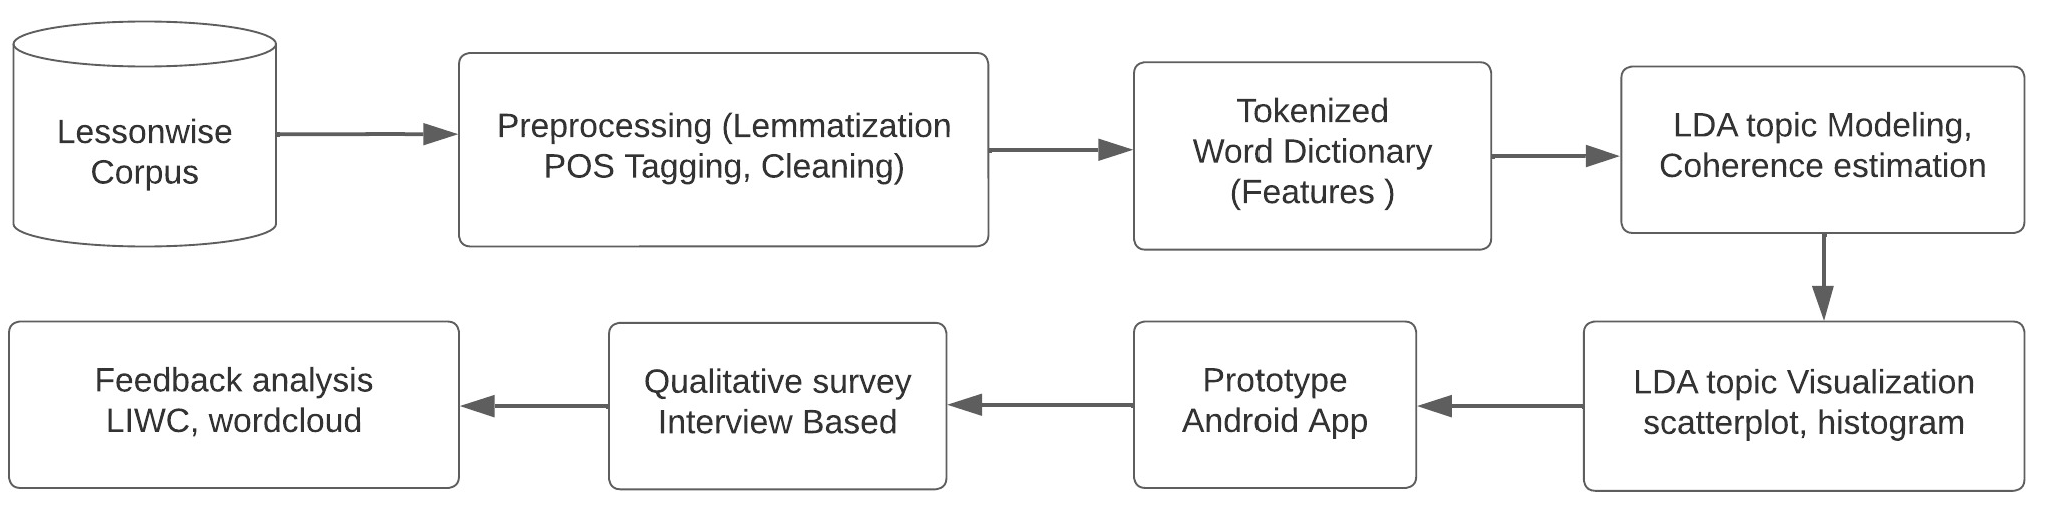
\includegraphics[width=0.9\textwidth]{methodology.png}
\caption{Research workflow diagram}
\end{figure}

LDA algorithm automatically discovers latent topics within the documents based on word co-occurrences. Each topic is represented by a set of words; interpret these words to understand the main concepts associated with each topic. Extensive exploratory analysis is conducted to visualize the topic modeling outputs. Analyze the topics generated by the model, which require manual review and adjustment to ensure the topics make sense. 

\subsection{Data Pre-Processing}\label{data_pre} 
Text is converted to Lowercased and Normalized to ensure consistent pre-processing \cite{kao_natural_2007}. 
\begin{enumerate}[label=(\roman*)]
\item \textbf{Data cleaning}: unwanted characters, punctuation, and special characters are removed, and stop words (such as "and," "the," "is," etc) are removed. The Spacy library's English word model and NLTK's stopword list are used together. Also, words less than two characters are removed, such as: I, Hi, Oh, etc. Hence, noise is removed, and irrelevant characters, symbols, or data artifacts that have been introduced during data collection or scraping from a pdf file to a text file are separated. Hence, we found a clean corpus. 
\item \textbf{Lemmatization}: Root words are collected words, and their dictionary form (lemma) is extracted using NLTK's WordNetLemmatizer package. Stemming reduces words to their base or root form, is not used since sometimes it changes the actual words. \item \textbf{Part-of-Speech Tagging}: Spacy's English model `en\_core\_web\_sm' is used to extract interested words (such as noun, verb, and adjective) and excluded (CCONJ, AUX, DET, INTJ, PART etc which are Coordinating Conjunction, Auxiliary, Determinator, Interjection, Particle, etc) thereby collecting tokens for only those that are not punctuation, conjunction, symbol, etc. \end{enumerate} 

\subsection{Topic Modeling and Feature Extraction}\label{top_mod_feature} Different techniques have been developed to perform topic modeling in the unsupervised topic modeling domain of Natural Language Processing (NLP), each with its own strengths and limitations \cite{vayansky2020review, abdelrazek2022topic, yi2009comparative}. Apart from LDA, Mallet LDA, Structural Topic Model (STM), Hierarchical Dirichlet Process (HDP), Non-Negative Matrix Factorization (NMF), Latent Semantic Analysis (LSA) etc are also prevailing and can be considered for comparative research studies. Prevailing LDA based data mining techniques are applied for feature extraction. 

\subsection{Latent Dirichlet Allocation (LDA)} \label{lda_mdel} 
LDA model \cite{jelodar_latent_2019, gupta_pan_lda_2021, pichardo_lagunas_svd_lda_2015, selvi_classification_2019} considers documents as mixes of topics, and each topic is a distribution over words. The objective is to derive the hidden topic assignments and the topic-word distributions that most effectively describe the observed documents. The goal of LDA is to uncover these latent topics from a collection of documents without needing any prior labeling or categorization of the content. An expression for the joint distribution of the LDA model is described below: \begin{equation} P(\theta_d,z,w\|\alpha,\beta)=P(\theta_d\|\alpha)\prod^N_{n=1}P(z_{d,n}\|\theta_d)P(w_{d,n}\|z_{d,n},\beta) \end{equation} Where $w_{d,n}$ the $n_{th}$ word in document $d$, $z_{d,n}$ the topic assigned to the $n_{th}$ word in document $d$, $\alpha,\beta$ are the Dirichlet LDA model parameters. controls per-document topic distribution and per-topic word distribution. $\theta_d$ represents the topic distribution. $P(\theta_d \| \alpha)$ Dirichlet distribution representing the document-topic distribution, $P(z_{d,n}\|\theta_d)$ is the word topic assignment for the $n_{th}$ word in document $d$, $P(w_{d,n}\|z_{d,n},\beta)$ is the distribution representing the observed word given a topic. An algorithm for the LDA model is explain below:


\begin{algorithm}[H]
    \caption{Latent Dirichlet Allocation (LDA)}
    \KwData{Documents $D$, Vocabulary $V$, Number of topics $K$}
    \KwResult{Document-topic distribution $\theta_d$, Topic-word distribution $\phi_k$}

    \textbf{Initialization:}\;
    Randomly assign each word in each document to one of $K$ topics\;

    \While{Not converged}{
        \textbf{
        Calculate probabilities:}\ 
        
        $\theta_{d, t} \propto \frac{\text{count}(z_{d, n} = t) + \alpha}{\sum_{t'} (\text{count}(z_{d, n} = t') + \alpha)}$\;
        $\phi_{t, w} \propto \frac{\text{count}(z_{d, n} = t, w) + \beta}{\sum_{w'} (\text{count}(z_{d, n} = t, w') + \beta)}$\;

        \textbf{
        Update distributions:}\
        $\theta_d \sim \text{Dirichlet}(\alpha + \sum_{n} \mathbb{I}(z_{d, n} = 1), \ldots, \alpha + \sum_{n} \mathbb{I}(z_{d, n} = K))$\;
        $\phi_k \sim \text{Dirichlet}(\beta + \sum_{d, n} \mathbb{I}(z_{d, n} = k, w_{d, n} = 1), \ldots, \beta + \sum_{d, n} \mathbb{I}(z_{d, n} = k, w_{d, n} = V))$\;

        \textbf{
        Reassign each word to a new topic:}\
        $z_{d, n} \sim \text{Multinomial}(\theta_{d,1}, \ldots, \theta_{d,K})$\;
    }

\end{algorithm}

We have chosen LDA as the baseline statistical topic modeling tool. An abstract of this model is depicted in figure~\ref{abstract_lda}
\begin{figure}[h!]
\centering
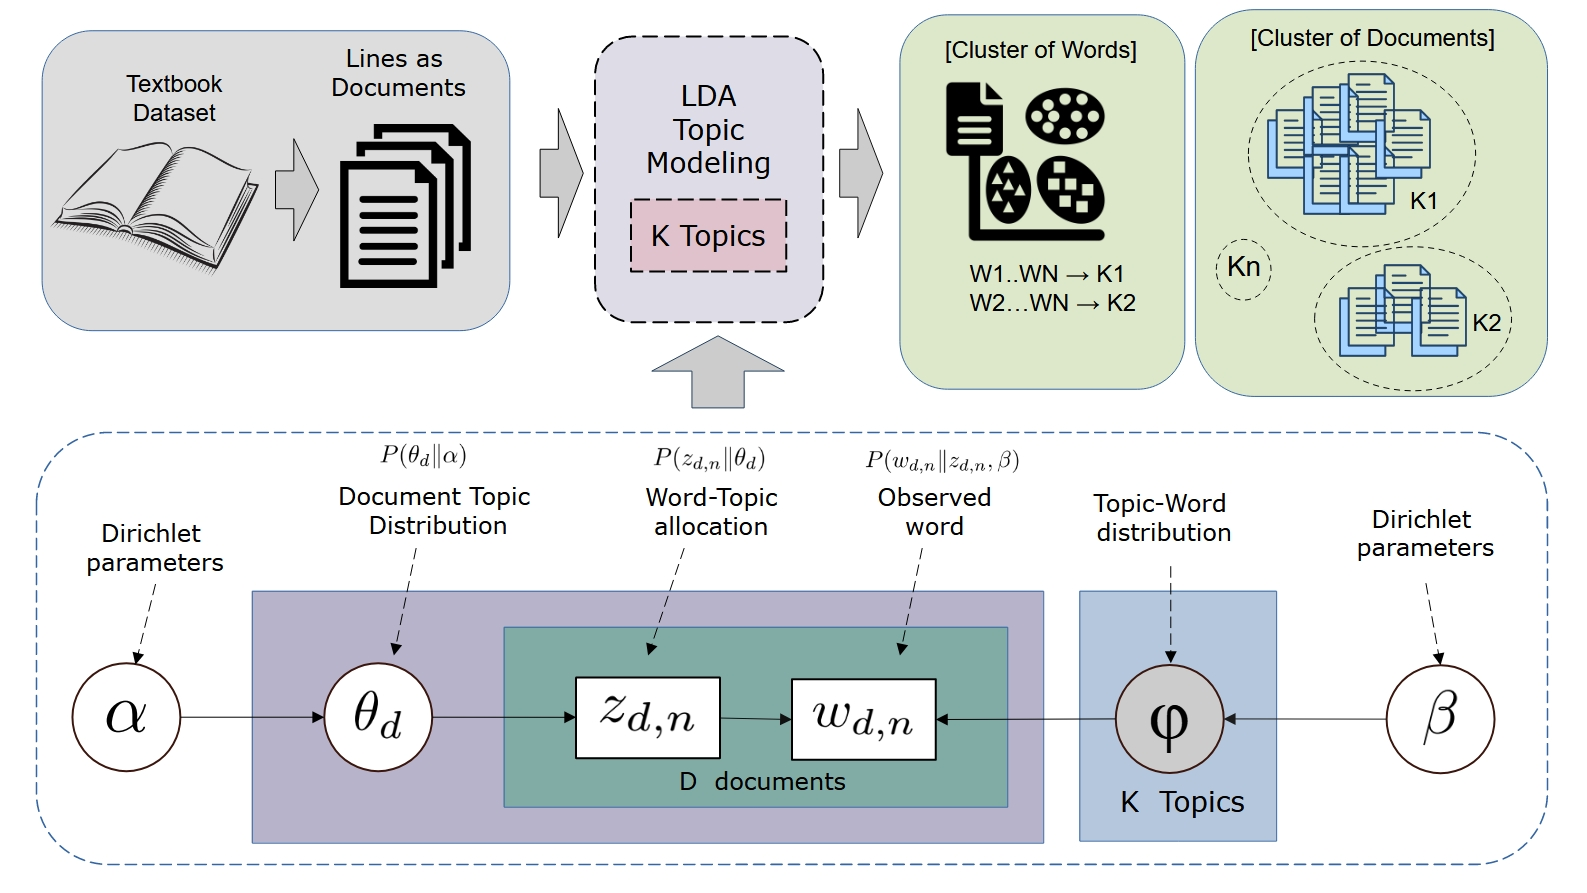
\includegraphics[width=0.9\textwidth]{lda.jpg}
\caption{Abstract LDA model workflow diagram}
\label{abstract_lda}
\end{figure}

\subsubsection{Comparative analysis of Topic modeling} 
While some variations of LDA, Mallet LDA is considered for large corpus processing and analysis \cite{vayansky2020review, abdelrazek2022topic, Comparison_Topic_Modeling_Algorithms}. It focuses on scalability. If large corpus needs to be analyzed, Mallet LDA might be more suitable. LDA in general can still be efficiently applied to moderately sized corpora. Analyzing topics within the context of metadata, STM could be a better fit. The Hierarchical Dirichlet Process (HDP) can be useful when we cannot guess the number of topics in advance. In \cite{Comparison_Topic_Modeling_Algorithms} LSI, NMF, and LDA are compared in terms of coherence and similarity measures for the social media dataset, and in their analysis, NMF is observed to be the most effective measure. However, as a baseline model, LDA is often considered one of the most prominent choices. In this study, the textbook corpus is divided into lessons, which are a mixture of topics, and using LDA, it is expected to be determined which words in the lesson belong to Lesson\textquotesingle s topics. LDA produces interpretative results for exploratory topic analysis. The identified topics are represented as distributions over words, making it easy to assign meaningful labels to topics. Provided by most of the libraries and tools, making it easy to implement and can be integrated into existing workflows. Hence, LDA serves as a solid baseline for topic modeling tasks. However, how many topics are ideal needs to be determined, and topic modeling quality also needs to be measured. 

\subsection*{LDA vs PCA: Mathematical Perspective}
LDA sometimes compared directly with PCA as a dimensionality reduction tool that identifies the principal components capturing maximum variance in the data.
\textbf{Covariance Matrix:}
\begin{equation}
    \Sigma = \frac{1}{N}\sum_{i=1}^{N}(X_i - \mu)(X_i - \mu)^T
\end{equation}

PCA represents data using the principal components, reducing dimensionality using Eigenvalue.

\textbf{Dimensionality Reduction:}
\begin{equation}
    Y = X \bm{V}
\end{equation}

where \(Y\) is the reduced-dimensional representation, \(X\) is the original data, and \(\bm{V}\) contains the principal components.

\textbf{Variance Preservation:}
\begin{equation}
    \frac{\sum_{i=1}^{k}\lambda_i}{\sum_{i=1}^{D}\lambda_i}
\end{equation}

PCA is effective for data compression and noise reduction widely used in scenarios where reducing the number of features is crucial, such as in image analysis or signal processing. LDA provides interpretable topics that can be useful for understanding the thematic structure of a document collection.


\subsubsection{Optimal Topics with Coherence} 
The coherence score measures how coherent or interpreted the words in that topic and estimates the number of topic clusters \cite{mimno2011optimizing}. The coherence score assesses the quality of the topics produced by LDA and ensures that the topics generated are statistically significant. Coherence \(C_{topic}\) can be expressed as follows: \begin{equation} C_{topic}=\sum^N_{i=1} \frac{1}{N(N-1)}\sum^i_{j=1} PMI(w_i,w_j) \end{equation} Where, \(PMI\left( w_{i},w_{j} \right)\) represent pointwise mutual information statistical association between two words occurring together. PMI score indicates that the two words are more closely related within a topic. \(PMI\left( w_{i},w_{j} \right)\) can expressed as \begin{equation} \(PMI\left( w_{i},w_{j} \right) = \log\frac{P\left( w_{i},w_{j} \right)}{P\left( w_{i} \right)P\left( w_{j} \right)}\) \end{equation} where \(P\left( w_{i},w_{j} \right)\) is joint probability of occurrence of words \(w_{i}\) and \(w_{j}\). To calculate the coherence score, the gensim library provides range of options such as \(u_{mass},c_{v},c_{uci},c_{npmi}\). \(u_{mass}\) and \(c_{v}\)These two methods are most popular. For given topic with words \(\{ w_{1},w_{2},w_{3},\ldots..,w_{n}\}\) a fixed context window size is provided (default size 10 words) then coherence score is calculated using an equation \(\sum_{j = 1}^{i}{PMI}\left( w_{i},w_{j} \right)\) which provides negative coherence score. \(c_{v}\) can be expressed as \begin{equation} \(c_{v} = \frac{1}{N(N - 1)}\sum_{j = 1}^{i}{similarity\left( w_{i},w_{j} \right)}\) \end{equation} in which \(similarity\left( w_{i},w_{j} \right)\) represent the pairwise similarity between terms based on \(PMI\left( w_{i},w_{j} \right)\) scores. \(c_{v}\) provides a positive coherence score. Higher coherence values (higher than 0.5) indicate that the topics are moderately coherent and representative of meaningful themes within the text data. 

\subsection{Visualize participants response}\label{vis_part} 
\subsubsection{Linguistic Inquiry and Word Count (LIWC)} \label{liwc}
In this research, LIWC is used to ascertain the general sentiment of the responses given by the survey participants (see section \ref{q_sentiment}). Linguistic Inquiry and Word Count (LIWC), is a text analysis tool to measure psychological or emotional characteristics \cite{tausczik2010psychological, liwc22_welcome_nodate}. It aims to quantify sentiment by examining the frequencies of different linguistic terms within given text based on predefined dictionary of words associated with various categories. Let's assume text as a sequence of words: \(\left\{ w_{1},w_{2},\ldots.,w_{n} \right\}\) and M different linguistic categories: \(\left\{ C_{1},C_{2},\ldots.,C_{m} \right\}\) . Proportion of words in each category \(P\lbrack i\rbrack = \frac{w\lbrack i\rbrack}{T}\) where T is the total number of Text. Now, a matrix \(X\lbrack i,j\rbrack\) can be formed, where \(w_{i}\) represents the frequency of the word in the linguistic category \(C_{j}\). LIWC vector containing the proportions of words in each linguistic category can be expressed as \(P_{total}\lbrack j\rbrack = \frac{\sum_{i = 1}^{T}{X\lbrack i,j\rbrack}}{T}\).

\subsubsection{Word cloud} \label{wordcloud} LIWC involves linguistic analysis using mathematical expressions, but using word clouds, survey answers can be visualized vividly in an interpretable interactive format. Word cloud consider a set of words \(\left\{ w_{1},w_{2},\ldots.,w_{n} \right\}\) extracted from text document and associated frequencies \(\left\{ f_{1},f_{2},\ldots.,f_{n} \right\}\), \(s_{i}\) represent the proportional size of the word in the cloud can be expressed as \(s_{i} = \frac{f_{i}}{\sum_{j = 1}^{n}f_{j}}\) where normalized frequency \(f_{i}\). In sections \ref{q_sentiment} figure \ref{word_cloud_1} and \ref{word_cloud_2} we can see the participants responses most frequent terms.

\section{Experiment and analysis}\label{exp_analysis} In this research study, for the dataset we have collected, Bangladesh NCBI provided an English textbook for classes 9–10. Here, the whole book is segregated into lessons, and we wanted to explore the important topics within the content. Similar topic words remain together. Therefore, assumptions are that it helps students understand the words, sentences, and context of the book. The ideal number of topics are determined using the coherence score \cite{mimno2011optimizing}. 

\subsection{Coherence measurements}\label{coh_measure} To measure coherence in the context of LDA, following steps are followed: 

\begin{enumerate}[label=(\roman*)] 
\item Cleaned document samples are prepared using Python's NLP data mining techniques explain in detailed in data reprocessing section. Prepared \(T\left( d_{i} \right)\) set of tokens in Documents \(d_{i}\) for \(i^{th}\) document samples in corpus \(D\). 
\item Doc to BOW corpus dictionary is prepared with a Doc2Bow vector. This vector \(x_{d}\) can be represented as where \(n\left( w_{i},d \right)\) denotes the count of words \(w_{i}\) for the document \(d\). 
\item Trained LDA Model: During the training phase, gensim's MulticoreLDA model with four CPU worker thread is set. Doc2Bow dictionary is applied, along with 20 iterations that are invoked. The rest of the parameters for LDA model training were the default parameter settings of gensim library. 
\item Calculate Coherence: To calculate the coherence score for each LDA model for \(n\) number of topics, step 3 is iterated for \(n = 15\) times. 
\item Iteration result coherence score for \(n\) number of topics are saved in a list and plotted using Seaborn. 
\end{enumerate} 

\begin{figure}[h!] \centering \begin{subfigure}{0.45\textwidth}
 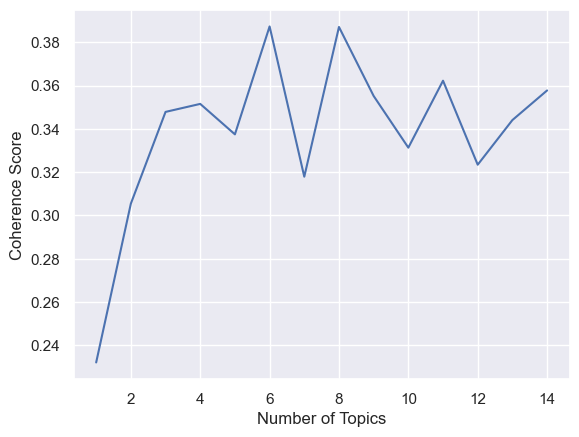
\includegraphics[width=\textwidth]{cv.png} \caption{Coherence for $c_v$ approach} 
 \end{subfigure}
  \hfill \begin{subfigure}{0.45\textwidth} 
 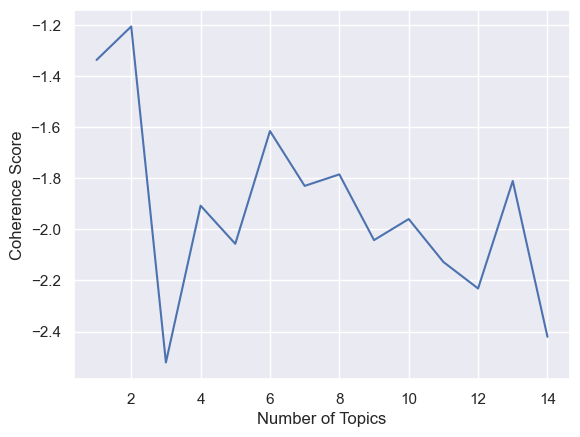
\includegraphics[width=\textwidth]{umass.png} \caption{Coherence for $u_{mass}$ approach} 
\end{subfigure} 
\caption{Coherence score to estimate optimal number of Topics} 
\label{cv_umass} 
\end{figure}

 From the chart we can see that six topics are dominant in our provided corpus. The chart shown at the left shows the coherence score for \(u_{mass}\) and the right chart represents the score for \(c_{v}\) for multiple iterations. Using 6 topics we can see the output of corresponding topic and top 10 words in a topic.

\begin{longtable}[]{@{}
  >{\raggedright\arraybackslash}p{(\columnwidth - 4\tabcolsep) * \real{0.17}}     
  >{\raggedright\arraybackslash}p{(\columnwidth - 4\tabcolsep) * \real{0.83}}@{}}
\toprule
Topics & Dominant Keywords and Weights \\
\midrule
\endhead
\textbf{Topic 01} & \enquote*{energy} 0.060, \enquote*{source} 0.029, \enquote*{renewable} 0.018, \enquote*{water}0.016, \enquote*{use} 0.013, \enquote*{gas} 0.013, \enquote*{produce} 0.013, \enquote*{green} 0.013, \enquote*{warm}
0.013, \enquote*{cause} 0.012 
\\
\textbf{Topic 02} & \enquote*{pastime} 0.024, \enquote*{computer} 0.024, \enquote*{social} 0.023, \enquote*{user} 0.022, \enquote*{network} 0.020, \enquote*{student} 0.019, \enquote*{class} 0.017, \enquote*{change} 0.016, \enquote*{book} 0.015, \enquote*{survey} 0.013  
\\
\textbf{Topic 03 }& \enquote*{mother} 0.083, \enquote*{buy} 0.021, \enquote*{love} 0.018, \enquote*{child} 0.014, \enquote*{worker} 0.014, \enquote*{begin} 0.013, \enquote*{cultural} 0.012, \enquote*{observe} 0.012, \enquote*{thing} 0.012, \enquote*{language} 0.011 
\\ 
\textbf{Topic 04} &  \enquote*{life} 0.016, \enquote*{Bangladesh} 0.016, \enquote*{family} 0.015, \enquote*{home} 0.014, \enquote*{root} 0.014, \enquote*{language} 0.014, \enquote*{country} 0.013, \enquote*{Pakistan} 0.010, \enquote*{war} 0.010, \enquote*{man} 0.009 
\\ 
\textbf{Topic 05} & \enquote*{country} 0.031, \enquote*{river} 0.022, \enquote*{India} 0.022, \enquote*{land} 0.021, \enquote*{boat} 0.015, \enquote*{small} 0.015, \enquote*{population} 0.015, \enquote*{lake} 0.013, \enquote*{group} 0.012, \enquote*{house} 0.011 
\\ 
\textbf{Topic 06} & \enquote*{job} 0.064, \enquote*{English} 0.023, \enquote*{learn} 0.021, \enquote*{teacher} 0.017, \enquote*{use} 0.016, \enquote*{dream} 0.016, \enquote*{think} 0.016, \enquote*{thing} 0.015, \enquote*{school} 0.014, \enquote*{education} 0.013\\
\bottomrule
\end{longtable}


\subsection{Dominant topic determination}\label{dom_topic}

In LDA models, each document is composed of multiple topics. But typically, some specific topics are dominant. The following experiment extracts this dominant topic for each sentence and shows the relative weight of the topic and the keywords. It estimated which document belongs predominantly to which topic. How frequently the words have appeared in the documents and the weights of each keyword in the same chart, words that occur in multiple topics, and the ones whose relative frequency is greater than the weight.

\subsubsection{Relative Importance measurement}

Word frequency $n(w_{j},d_{i})$ in each document \(D\) is measured in equation \ref{eq:rela_weight} as below which identifies the most frequent words within each document and across the entire corpus.

\begin{equation}
\label{eq:rela_weight}
D = \sum_{d_{i} \in D}^{}\left\{ \begin{array}{l}
1,n\left( w_{i},d_{i} \right) > 0 \\
0,n\left( w_{i},d_{i} \right) = 0 \\
\end{array} \right.\
\end{equation}

we can visualize relative importance of any keywords in terms of frequency and plotted inclined with LDA provided weights (figure \ref{fig:Relative_weight}).

\begin{figure}[h!]
\centering
%\includegraphics[width=18cm, height=10cm,angle=90]{Figs/relative_imp.png}
\includegraphics[width=\textwidth]{relative_imp.png}
\caption{Word frequency and its relative importance}
\label{fig:Relative_weight}
\end{figure}


\subsection{Topic-Term Matrix Visualization}\label{top_term_vis}

Visualizing the topics and their relationships in a topic model The Python library PyLDAvis is used to provide an interactive web-based interface to explore and analyze the LDA results of topic modeling. PyLDAvis itself abstracts away much of the underlying mathematical complexity and provides a user-friendly way to generate visualizations and interactively explore topics and their relationships. Key components of distance among topics and salient terms are explained below:

\subsubsection{Inter-Topic Distance Map}

Distance among topics refers to the measurement of similarity between topics in a high dimensional space matrix provided by the LDA model. PyLDAvis library is used to conserve dimensionality reduction using PCA and for calculating distance between topics metric like Euclidean distance or Cosine Similarity. 

\subsubsection{Salient Terms or dominant keywords} Salient terms in a topic are words \(W\) that are most strongly associated with a specific topic. The mathematical expression for finding salient terms \(w\) for a topic \(t\) involves the extraction of top \(n\) words that pose the highest probability scores for topic \(t\) in the topic-term matrix \(P\lbrack t,w\rbrack\).

\begin{figure}[h]
\centerline{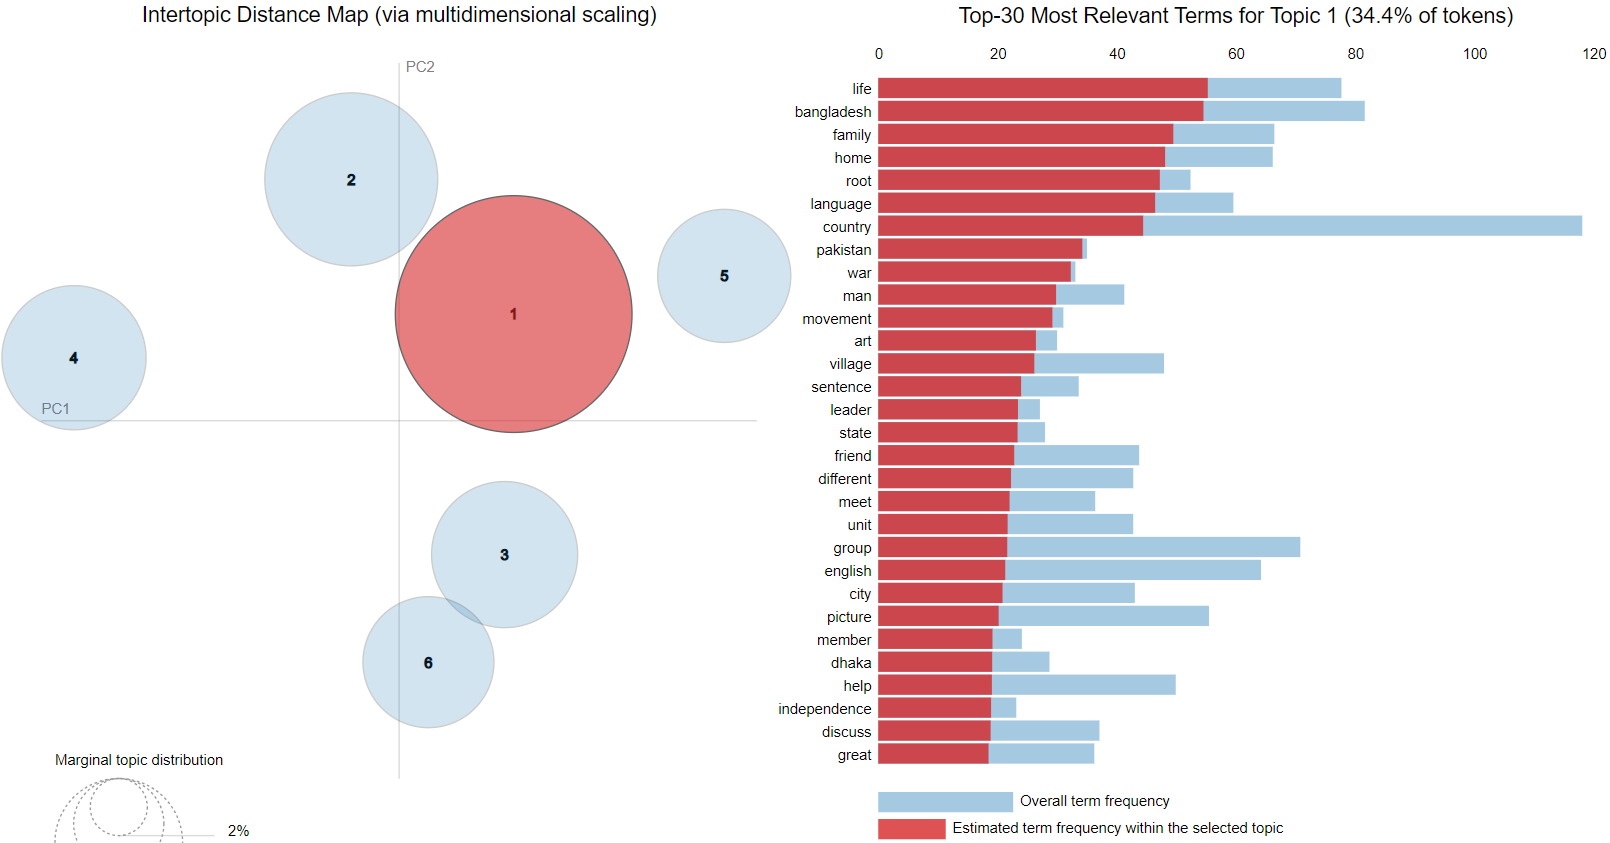
\includegraphics[width=\textwidth]{pyldvis.png}}
\caption{Topic model co-occurrence visualization with dominant keywords'}
\label{Relative_weight_pyldvis}
\end{figure}

The top 30 most salient terms are shown at right in the bar chart histogram, and the left figure shows inter-topic distance, their size, etc. (see figure~\ref{Relative_weight_pyldvis}). The PCA dimensionality reduction technique is applied here to embed the LDA result into a 2D plain scale. Projecting the data in lower-dimensional subspace by computing eigenvalues reduced the circle overlapping. Topics that are closer together in the map are more similar in terms of the distribution of words. 

\subsection{Qualitative survey}\label{qual_survey} In the survey questions, it was indicated whether the students, teachers, and government organizations would find it acceptable and appreciated if textbook information were made available through a mobile app and presented in interactive format. To demonstrate the mobile app idea during the interrogation survey session, a prototype app, Englisher, is prepared (see demo in Section \ref{Englisher_mobile_app}). Participants were asked for suggestions on how to make the app better and to specify shortcomings. Presumably It provides an insight into teacher’s emotions about the inclusion of mobile technology in the higher secondary English education system.

\subsubsection{Englisher Mobile App}
\label{Englisher_mobile_app}
A mobile application (Englisher) is being developed with content from the NCTB’s English Textbook for class 9. The extracted keywords are organized into lessons, and furthermore, a quiz is introduced as an exercise. Each sentence's and word's Bengali meanings are provided in accordance with the lesson. Students can take quizzes, and their results are recorded in history so that history can be reviewed and performance can be improved with more practice in the future.

\begin{figure}[h!]
\centering
\begin{subfigure}{\textwidth}
	\centering
    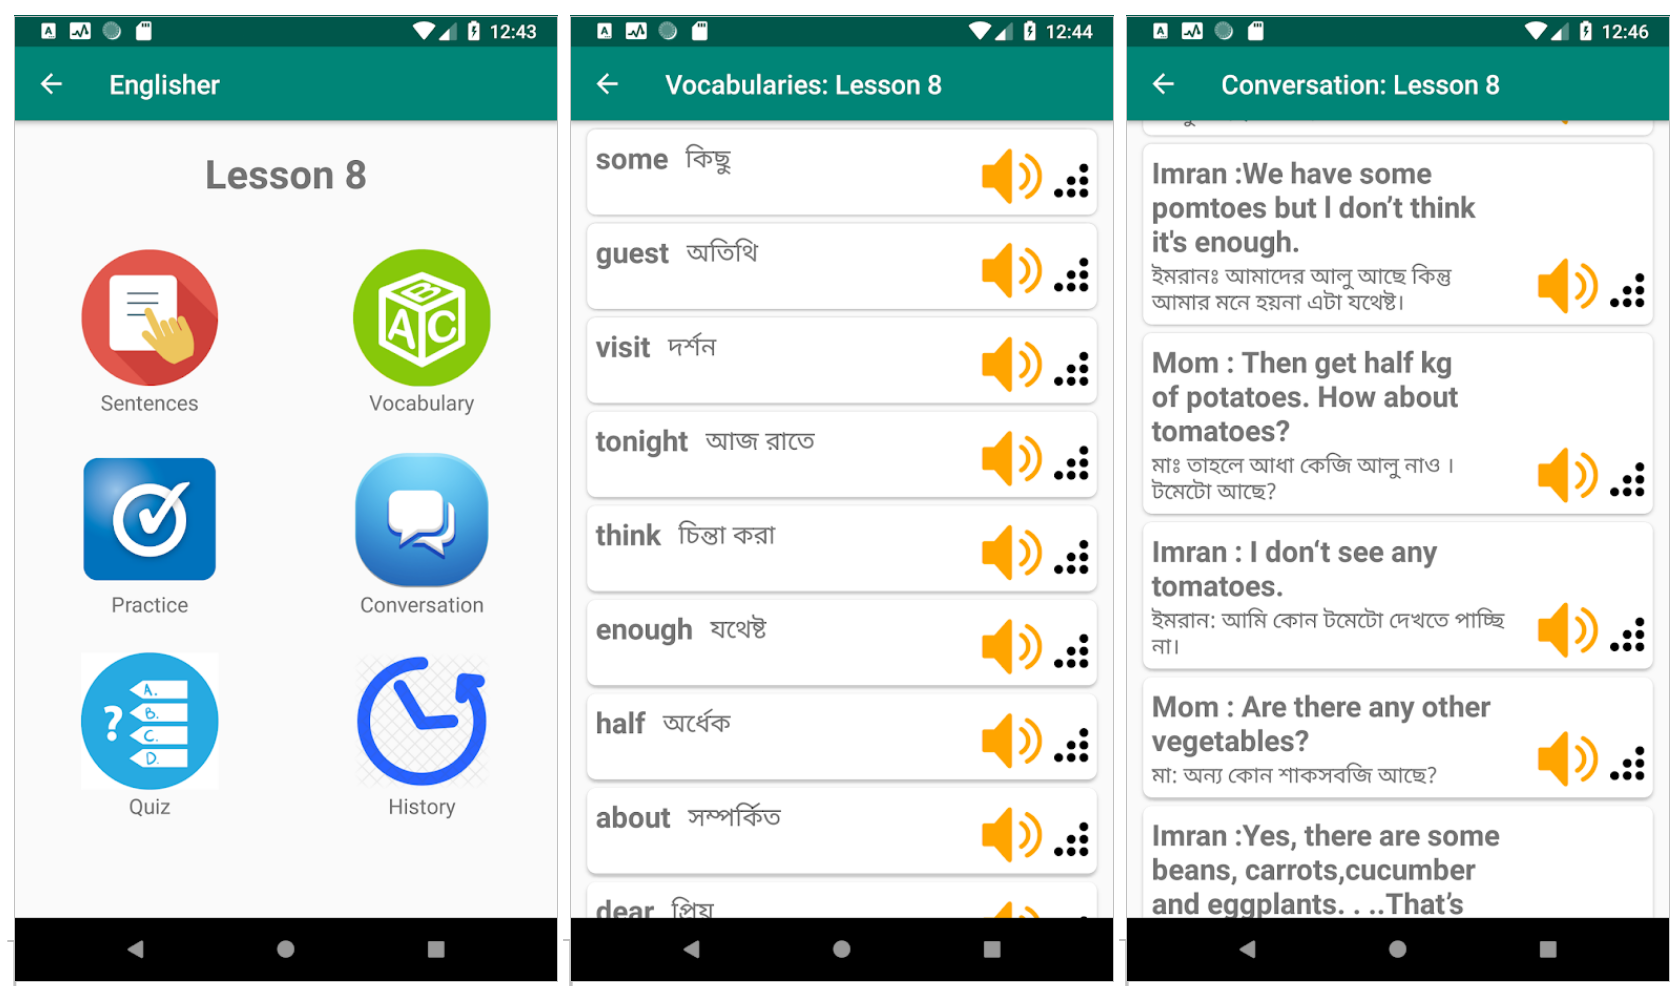
\includegraphics[width=\textwidth]{mobile_app_01.png}
    \caption{Lesson wise exercise}
    \label{fig:first}
\end{subfigure}
\hfill
\begin{subfigure}{\textwidth}
	\centering
    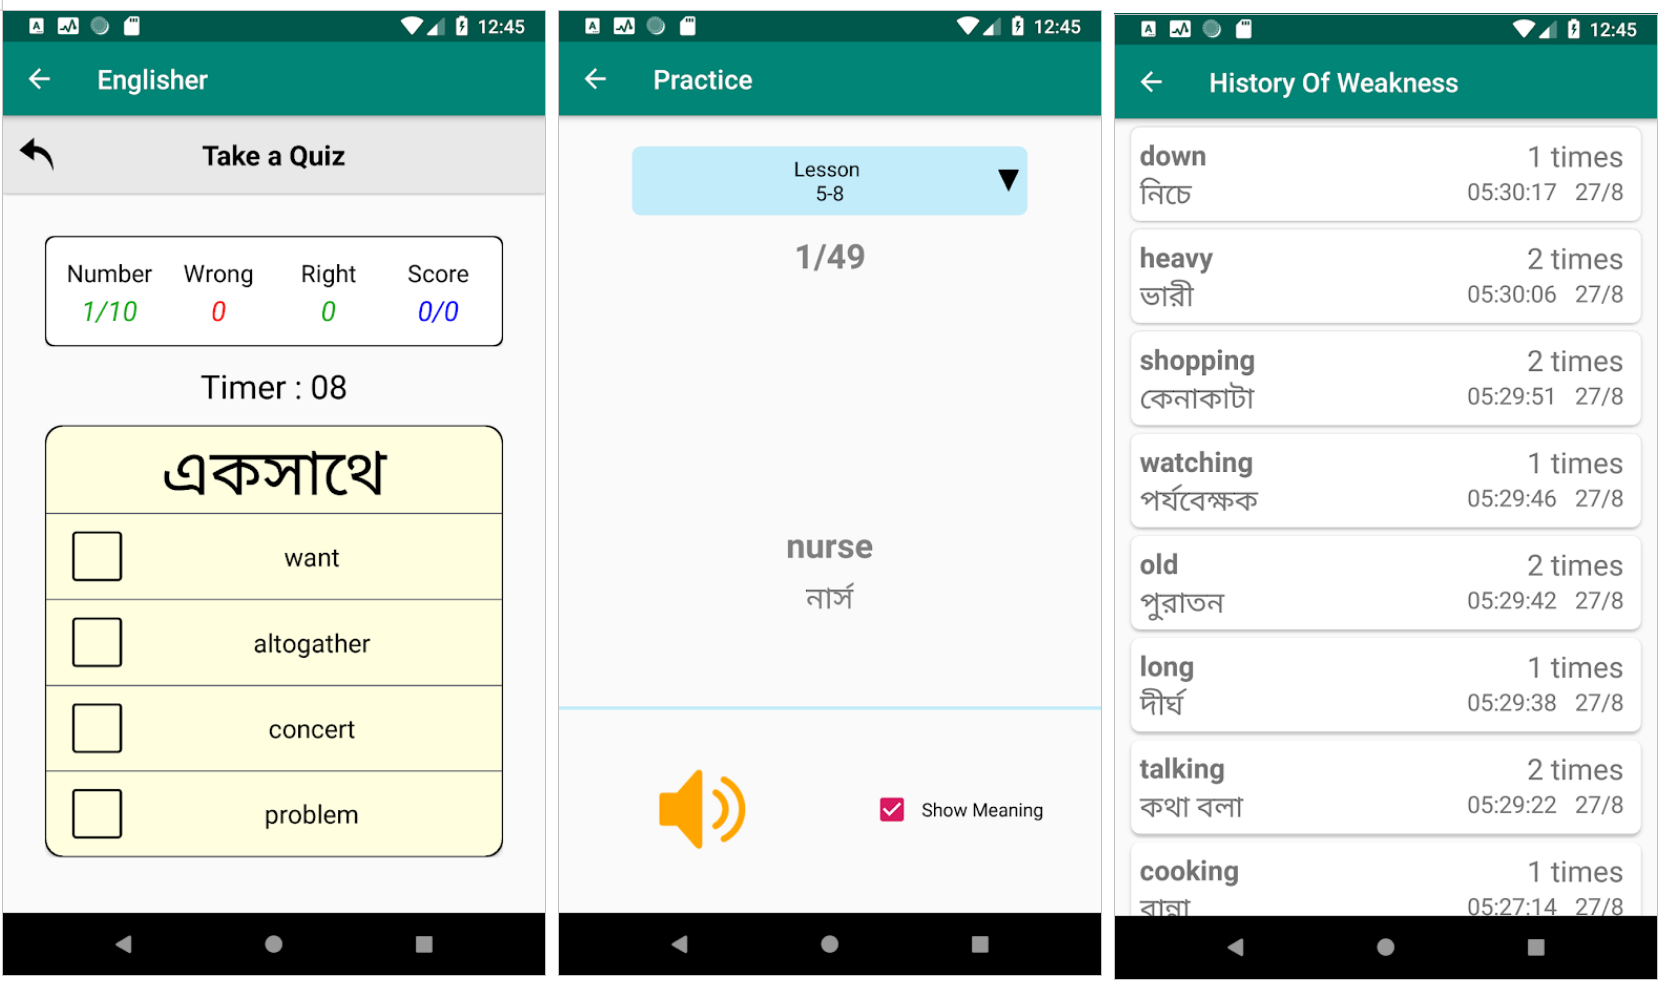
\includegraphics[width=\textwidth]{mobile_app_02.png}
    \caption{Quiz with Vocabulary}
    \label{fig:second}
\end{subfigure}
        
\caption{Englisher Mobile app for Learning LDA based topic model words}
\label{fig:figures}
\end{figure}

\subsubsection{Survey Planning} The survey was conducted over a period of four weeks with 50 high schools in Dhaka and Bogura districts of Bangladesh. It encompasses only English subject areas Teachers who teach in high schools from grade six to grade ten and teaches regularly in the school. A questionnaire was distributed to teachers, allowing us to gather answers. 

\subsubsection{Participants} During the survey, standard participants were chosen emphasizing infrastructure quality, teaching experience, class size, etc. At the beginning, 100 institutions were selected. Then half of them were excluded since the infrastructure's overall quality and condition were not above average. Among the chosen samples, 76\% were good and 26\% considered average institutions. Privately held 45\%, 32\% partially government, and 22\% are government institutes. Over 1000 students study in almost 40\% of these institutions, and a sizable number of pupils are present in each section and class. 38\% class have a size greater than 50. So, we can presume that the participating teachers have quite a bit of experience teaching a sufficient number of students. 

\subsubsection{Survey Results} We have done extensive analysis with the survey data collected. In our data collection, the highest priority is given to the secondary class student teachers who teach between 6 and 10th grade, about 46\%. High school, KG college, and KG high school. Details about the statistics are depicted in the following figures. Adjacent chart explains the percentage of teachers who teach in which class. Hence, from these two figures, we can get a vivid image of collected dataset resources about the participating teachers.

\begin{figure}[h!]
\centering
\begin{subfigure}{0.48\textwidth}
    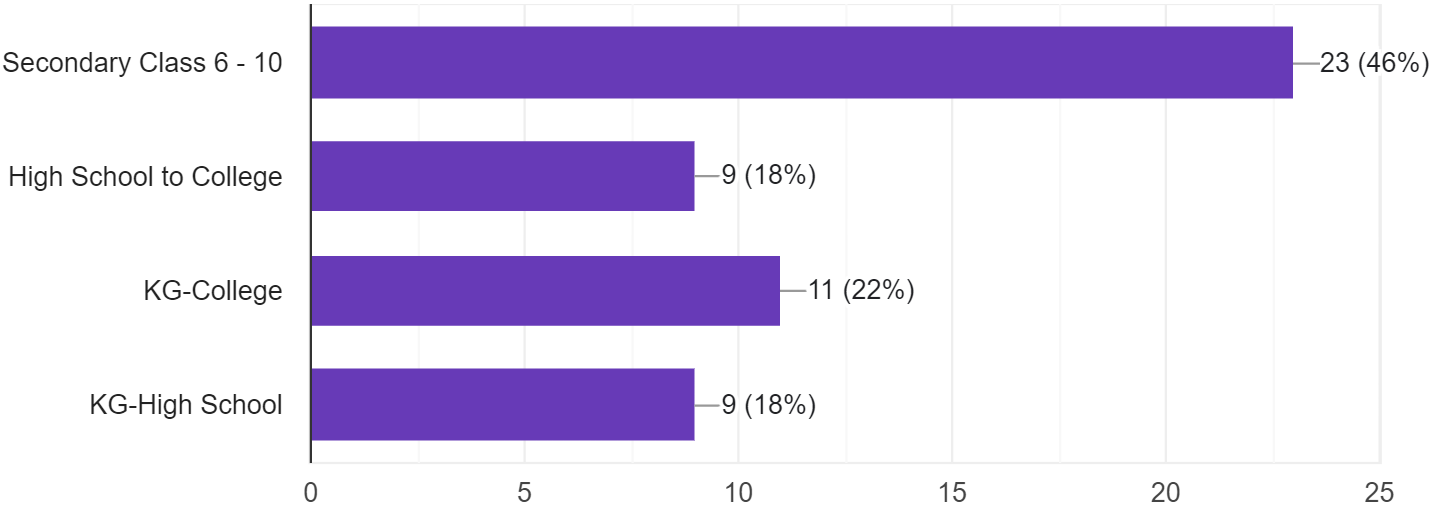
\includegraphics[width=\textwidth]{institution_size.png}
    \caption{Participating institution category and size}
    \label{cv}
\end{subfigure}
\hfill
\begin{subfigure}{0.48\textwidth}
    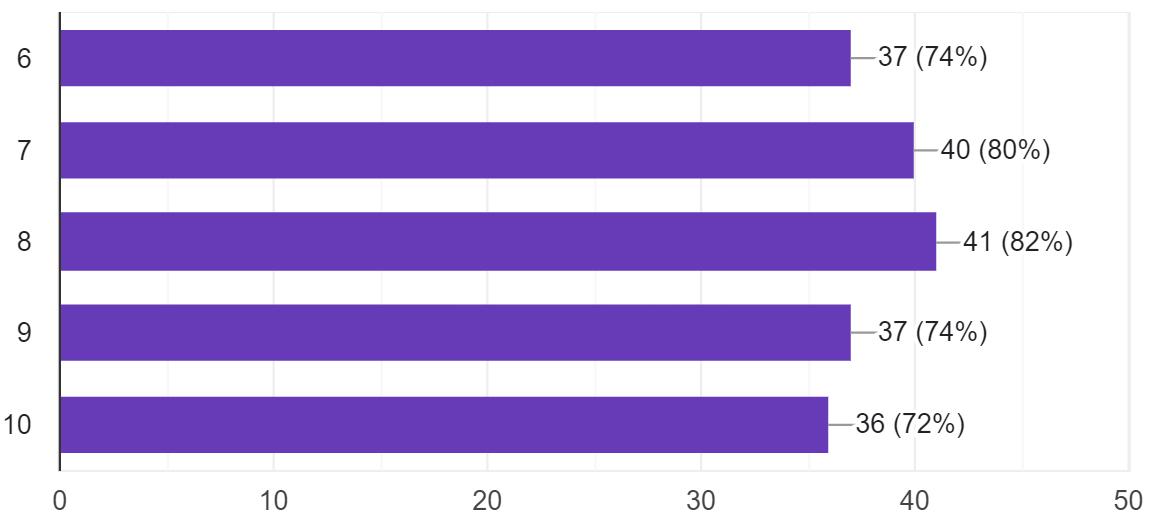
\includegraphics[width=\textwidth]{english_teaching_class.png}
    \caption{Participating instructors' class/Label}
    \label{umass}
\end{subfigure}       
%\caption{Coherence score to estimate optimal number of Topics}
\label{cv_umass}
\end{figure}

The following graphs give an overview of the English teaching experiences of the teachers as well as the general consensus regarding the use of digital content and mobile apps in everyday teaching and learning. Almost 62\% of teachers have been teaching for more than 8 to 10 years, and some of them have been teaching for decades in higher secondary education. 32\% of teachers have three to eight years of experience, while just 6\% are new to the profession. Around 83.7\% of teachers said the language of instruction during their graduation was English, and their major was also English. Very few teachers 13.3\% graduation major is something other than English, yet teachers teaching English in secondary schools probably have sufficient English language proficiency.

\begin{figure}[h!]
\centering
\begin{subfigure}{0.48\textwidth}
    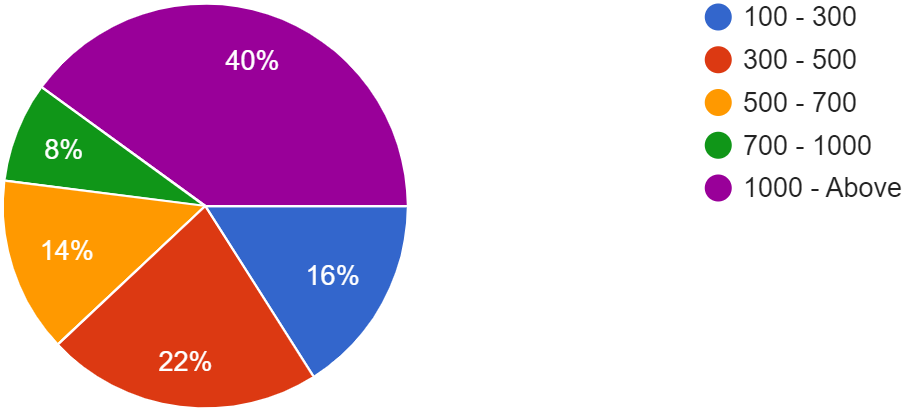
\includegraphics[width=\textwidth]{num_stu.png}
    \caption{Participating institutions' number of students}
    \label{cv}
\end{subfigure}
\hfill
\begin{subfigure}{0.48\textwidth}
    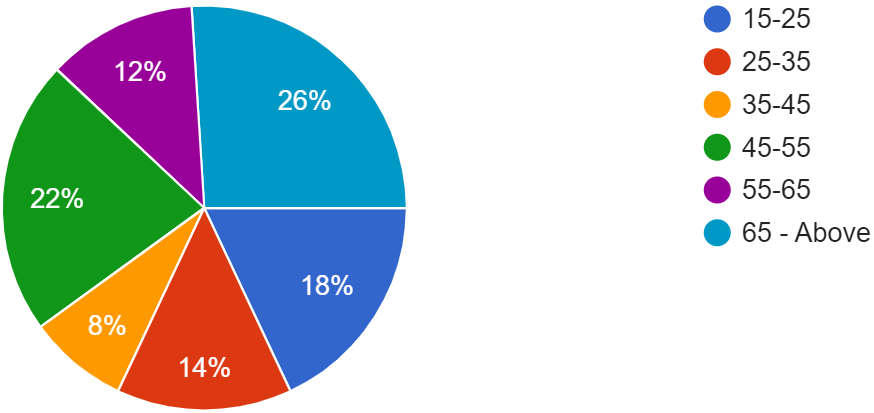
\includegraphics[width=\textwidth]{class_size.png}
    \caption{Participating instructors' class size}
    \label{umass}
\end{subfigure}       
%\caption{Coherence score to estimate optimal number of Topics}
\label{cv_umass}
\end{figure}

\subsubsection{Analyzing survey Facts} 
More than half of teachers, or 58\%, have no prior experience utilizing mobile apps or technology for teaching, but 90\% of them agree, and more than 45\% strongly agree, that it encourages pupils to engage actively in their learning. However, they (almost 60\%) also hold the opinion that a notebook cannot be completely replaced, despite the fact that mobile apps may solve many problems and provide technological support for teaching and learning. Promisingly optimistic approximately 40\%, although thinking that the notebook-based content memorizing learning method can be replaced, feel that mobile app-based learning can replace it permanently. 

\begin{figure}[h!]
\centering
\begin{subfigure}{0.48\textwidth}
    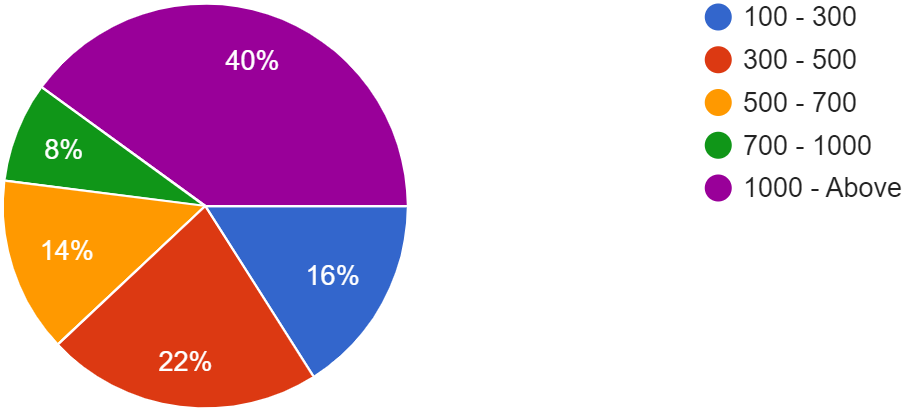
\includegraphics[width=\textwidth]{num_stu.png}
    \caption{Participating institutions' number of students}
    \label{cv}
\end{subfigure}
\hfill
\begin{subfigure}{0.45\textwidth}
    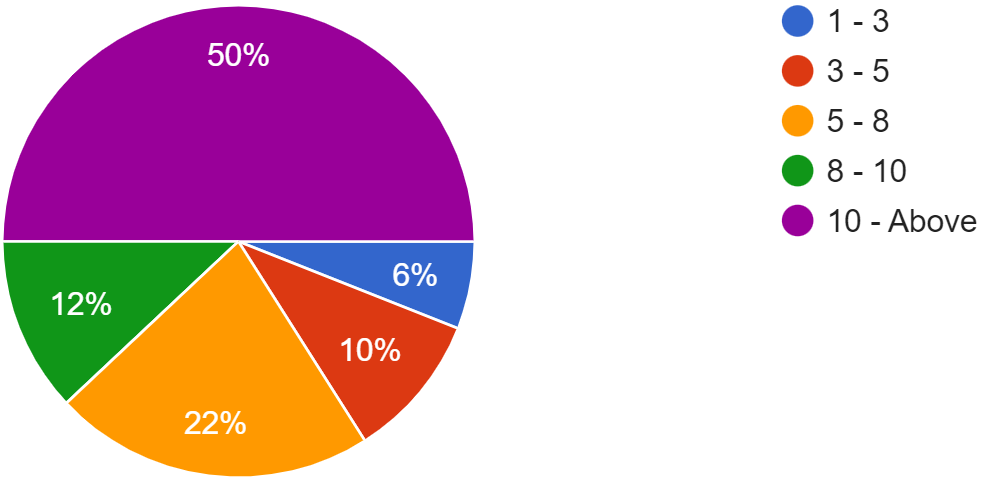
\includegraphics[width=\textwidth]{experience.png}
    \caption{Participating instructors' Teaching experience}
    \label{umass}
\end{subfigure} 
\begin{subfigure}{0.44\textwidth}
    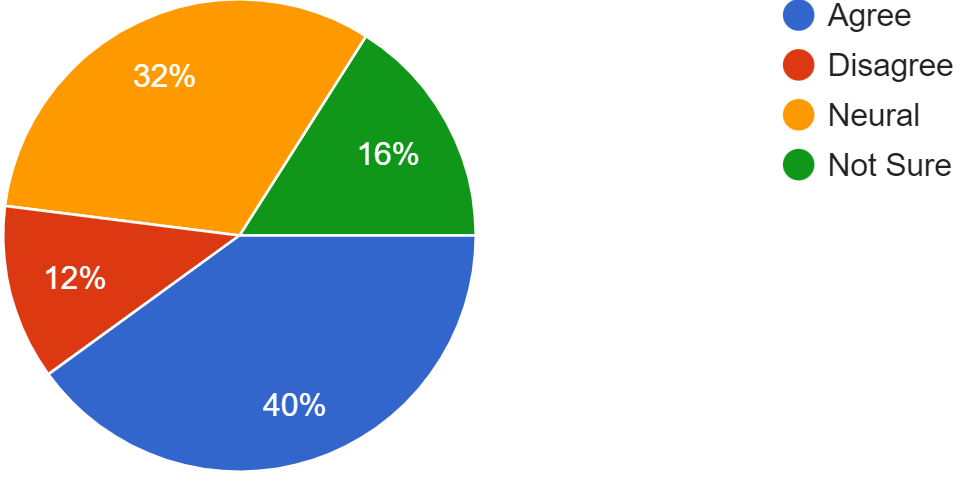
\includegraphics[width=\textwidth]{replace.png}
    \caption{App could help students in replacement of guide book}
    \label{cv}
\end{subfigure}
\hfill
\begin{subfigure}{0.47\textwidth}
    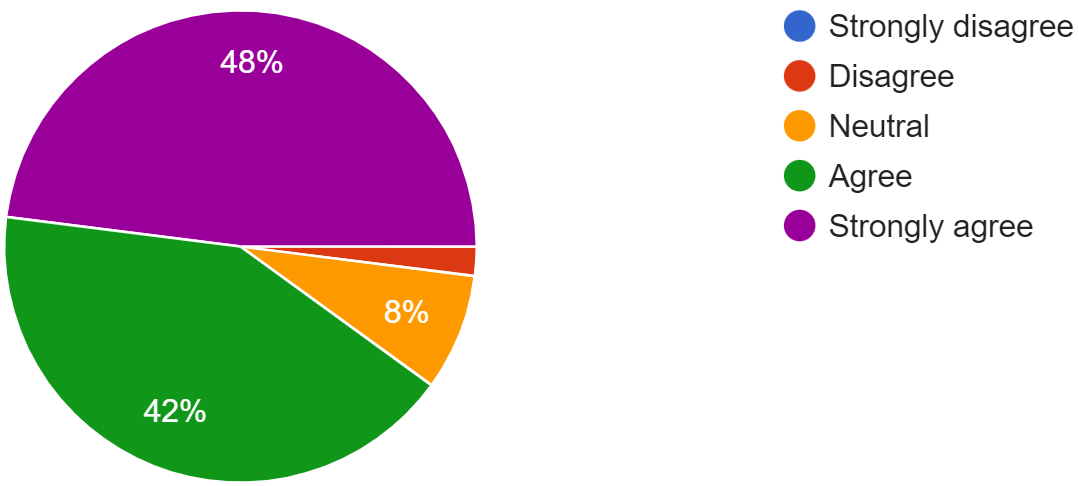
\includegraphics[width=\textwidth]{app_motivates.png}
    \caption{App could motivate students}
    \label{umass}
\end{subfigure}        
%\caption{Coherence score to estimate optimal number of Topics}
\label{cv_umass}
\end{figure}

This study proposes the Englisher mobile app and presents it to the participating teachers to gather their insightful feedback. 92\% of teachers reported that they would use this type of mobile app for teaching if it were made available after using the trial version of the offered customized Englisher app. Teachers anticipate that 80\% of students will utilize this app during class. 86\% of respondents believed it may help students' English proficiency, and 98\% agreed that the government should support this kind of innovation in the education sector. 

\begin{longtable}[]{@{}
  >{\raggedright\arraybackslash}p{(\columnwidth - 4\tabcolsep) * \real{0.7732}}
  >{\raggedright\arraybackslash}p{(\columnwidth - 4\tabcolsep) * \real{0.1066}}
  >{\raggedright\arraybackslash}p{(\columnwidth - 4\tabcolsep) * \real{0.1203}}@{}}
\toprule
\begin{minipage}[b]{\linewidth}\raggedright
\textbf{Questions}
\end{minipage} & \begin{minipage}[b]{\linewidth}\raggedright
\textbf{yes}
\end{minipage} & \begin{minipage}[b]{\linewidth}\raggedright
\textbf{No}
\end{minipage} \\
\midrule
\endhead
Do you use digital content for teaching or digital medium for teaching
and learning? & 84\% & 16\% \\
Have you ever used Internet or Mobile app to teach students or asked
students to find learning materials from internet or Mobile App? & 76\% &
24\% \\
Education during graduation was English and English was used for
learning & 83.70\% & 16.30\% \\
\multicolumn{3}{@{}>{\raggedright\arraybackslash}p{(\columnwidth - 4\tabcolsep) * \real{1.0000} + 4\tabcolsep}@{}}{%
\textit{Customized mobile app for Learning and Teaching English}} \\
Do you think topic model based mobile app-based learning can improve
English proficiency of students? & 86\% & 14\% \\
Do you think Govt should promote these types of innovation for education
sector? & 98\% & 2\% \\
\bottomrule
\end{longtable}

  \subsubsection{Qualitative Survey Sentiment}
  \label{q_sentiment}

\begin{longtable}[]{@{}
  >{\raggedright\arraybackslash}p{(\columnwidth - 12\tabcolsep) * \real{0.1709}}
  >{\raggedright\arraybackslash}p{(\columnwidth - 12\tabcolsep) * \real{0.1042}}
  >{\raggedright\arraybackslash}p{(\columnwidth - 12\tabcolsep) * \real{0.1794}}
  >{\raggedright\arraybackslash}p{(\columnwidth - 12\tabcolsep) * \real{0.1045}}
  >{\raggedright\arraybackslash}p{(\columnwidth - 12\tabcolsep) * \real{0.1756}}
  >{\raggedright\arraybackslash}p{(\columnwidth - 12\tabcolsep) * \real{0.1016}}
  >{\raggedright\arraybackslash}p{(\columnwidth - 12\tabcolsep) * \real{0.1638}}@{}}
\toprule
\begin{minipage}[b]{\linewidth}\raggedright
\textbf{Traditional LIWC Dimension}
\end{minipage} & \begin{minipage}[b]{\linewidth}\raggedright
\textbf{Answer Text}
\end{minipage} & \begin{minipage}[b]{\linewidth}\raggedright
\textbf{Standard Commercial Language}
\end{minipage} & \begin{minipage}[b]{\linewidth}\raggedright
\textbf{Answer Text}
\end{minipage} & \begin{minipage}[b]{\linewidth}\raggedright
\textbf{Standard for Formal Language}
\end{minipage} & \begin{minipage}[b]{\linewidth}\raggedright
\textbf{Answer Text}
\end{minipage} & \begin{minipage}[b]{\linewidth}\raggedright
\textbf{Standard for story language}
\end{minipage} \\
\midrule
\endhead
\textbf{Positive Tone} & 2.54 & 3.96 & 3.91 & 2.33 & 3.22 & 2.18 \\
\textbf{Negative Tone} & 0 & 1.1 & 0 & 1.38 & 0 & 1.75 \\
\textbf{Social Words} & 2.54 & 6.87 & 5.65 & 6.54 & 4.08 & 10.5 \\
\textbf{Cognitive Processes} & 13.56 & 9.35 & 18.26 & 7.95 & 15.88 &
8.7 \\
\textbf{Allure} & 2.54 & 7.79 & 3.04 & 3.58 & 2.79 & 5.48 \\
\textbf{Moralization} & 0 & 0.2 & 0 & 0.3 & 0 & 0.21 \\
\bottomrule
\end{longtable}

From this LIWC table, a higher proportion of words related to positive emotions indicates a positive emotional tone in the text in the answer to the questions related to ``How this app can be improved'' and ``How English learning can be improved using a mobile app''. LIWC is applied to three different categories: ``commercial writing'', ``Formal language'', and ``story language'', and in all the categories, the answer text showed highly positive sentiment from the survey user. Though respondents had a mix of optimism and skepticism regarding the use of mobile apps in teaching and learning,. During the interrogation session, their tone was positive and enticed participants.


\begin{figure}[h!]
\centering
\begin{subfigure}{0.48\textwidth}
    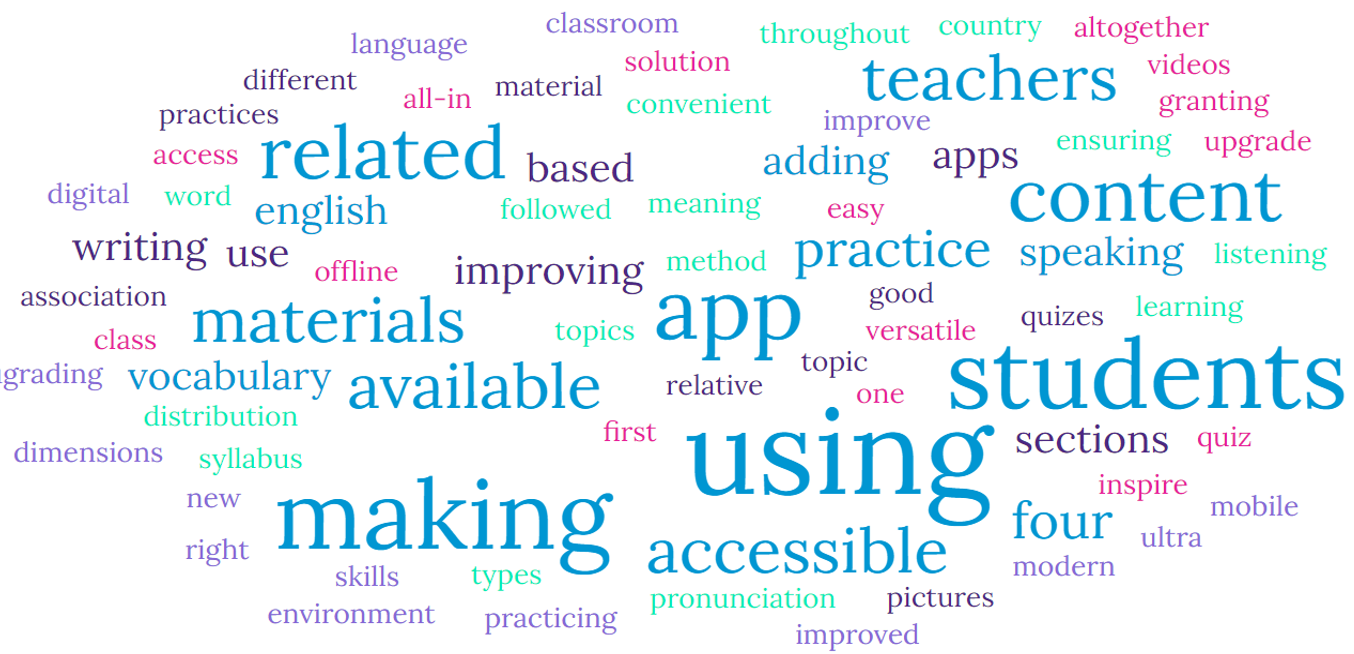
\includegraphics[width=\textwidth]{app_impv.png}
    \caption{word cloud for the question regarding app improvement}
    \label{word_cloud_1}
\end{subfigure}
\hfill
\begin{subfigure}{0.48\textwidth}
    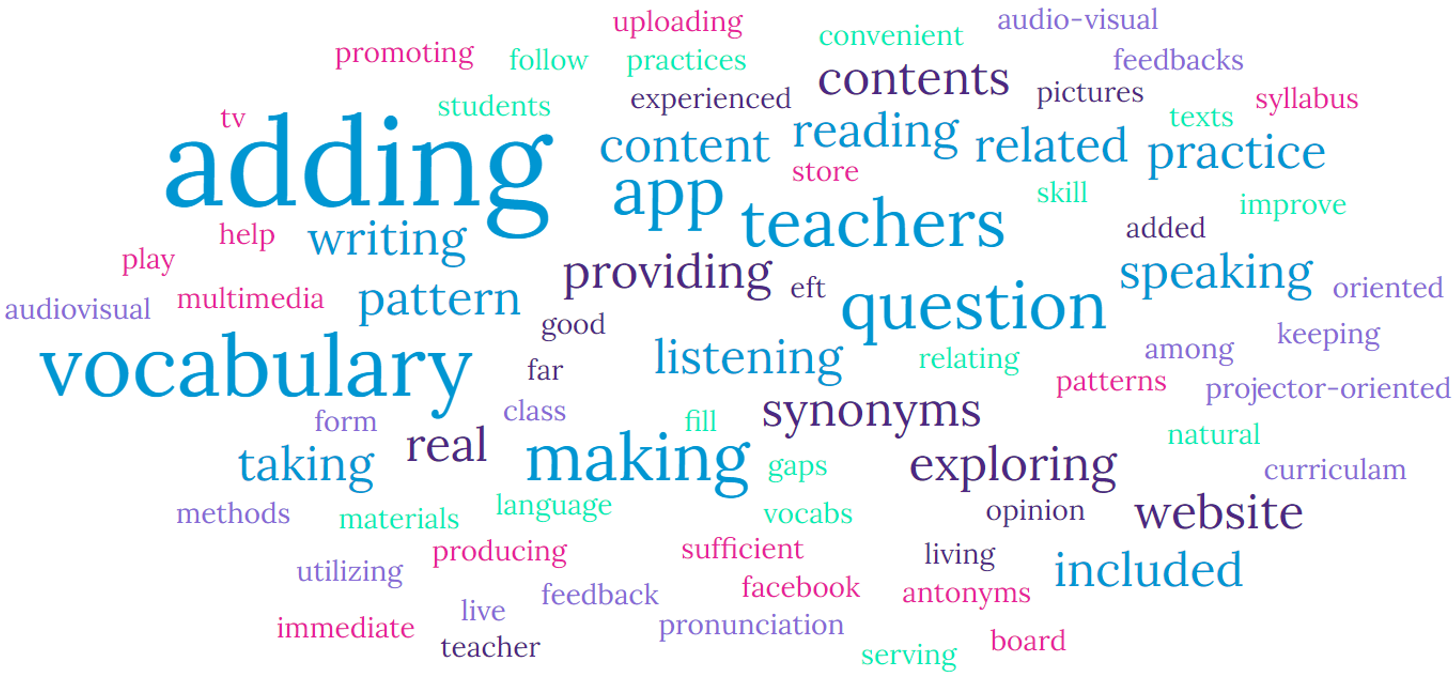
\includegraphics[width=\textwidth]{eng_app_impv.png}
    \caption{word cloud for the question regarding English learning app improvement}
    \label{word_cloud_2}
\end{subfigure}       
%\caption{Coherence score to estimate optimal number of Topics}
\end{figure}

The word cloud is generated from the answers provided to the question ``how the app can be improved'' and followed by a more generalized question ``how English learning can be improved using an app''. The participants narrated a variety of viewpoints on the questions. From the word cloud, it is inferred that adding graphical content would enhance the apps\textquotesingle{} usefulness and make them more visually appealing to users. More practice resources for listening and exercise would be helpful. Another suggestion is to include synonym and syllabus-related instances as well as audiovisual engagement with the app. Add additional vocabulary and involve more experienced teachers who have greater experience in digital learning and teaching.

\section{Results Discussion and outcomes}\label{res_dis}
The results demonstrate that LDA-based topic modeling significantly enhances content comprehension by providing concise summaries of the learning material. Readers can grasp the main ideas and connections between topics, aiding in retention and knowledge acquisition. From the qualitative survey, it was revealed that LDA based topic modeling approaches based on extracted keywords within mobile apps seem effective as they provide more contextual meaning to the learners. Most of the participating teachers are enthusiastic about topic modeling-based contextual resource learning related to technology incorporated into pedagogy. Participants appreciated the cutting edge NLP's learning resources available through mobile devices. Teachers admitted that available digital resources facilitated a deeper understanding of topics and catered to different learning styles, nurturing a more engaging learning environment. This will positively impact student motivation and overall engagement and, hence, boost overall learning. Some crucial suggestions were to improve the graphics of the app so that it becomes interactive and guardian involvement can be introduced. Based on the survey results, it is revealed that the potential for digital mobile-based learning in schools is immense. The government should take initiatives to incorporate it into the course curriculum syllabus and could impose an obligation to adopt mobile app-based learning teaching in the school.

Apps need to be improved by including collaborative form of learning.Additionally, the interactive interface receives positive feedback for its user-friendly design and utility in assistingreaders\textquotesingle{} navigation through the textbook.The recommendation is to make it specific to NCTB books only for particular classes. This approach is also our goal, considering NCTB Books. Including interactive e-books, dictionaries, educational apps, and multimedia content.

\section{Limitations}\label{limitat}

LDA could play a role in understanding the topics covered in an English textbook and potentially aiding in content customization and topic relevance for personalized learning. In a personalized learning context, the goal is to tailor the educational experience to the individual needs and preferences of each learner. This involves understanding the learner\textquotesingle s strengths, weaknesses, interests, and learning style. While LDA could be useful in some aspects of this process, it might not directly address all the requirements of personalized learning for an English textbook. In this research study, we showed that LDA based topic modeling could be a solution to enhance the context understanding of the learners. However, from the survey, it was revealed that the app was not sufficient. Learner oriented topic-document distribution to identify which topics are most relevant to a specific student can be provided. The app can provide additional explanations, examples, or resources to cater to their individual learning style. Assessments and exercises focused on the topics that need reinforcement for each student. Monitor their progress and adjust the learning path accordingly. Analyze students\textquotesingle{} performance, engagement, and feedback to refine the topic modeling process and its integration into the learning environment. More sophisticated approaches, such as adaptive learning systems and AI-based tutoring, might be needed to truly personalize the learning experience in a comprehensive manner.

\section{Special Remarks}

For data privacy and security issues, many teachers were reluctant to provide their social website addresses to the surveyor. Among all the participants, only 24\% attendees provided their social media addresses to use them publicly for research purposes.

\section{Conclusion}\label{conclu}
By employing topic modeling in a personalized learning context, educators can create a more engaging and effective learning experience. This approach allows for enhanced understanding and retention of the textbook context. The school survey with the prototype app reaffirmed its potential in learning experiences. LDA based topic modeling leverages learning experience to improve interpretation and knowledge acquisition. The synthesis of existing research sheds light on the potential of topic modeling to improve textbook context comprehension and the knowledge retention of learners. It was revealed that teachers and instructors would find it acceptable and appreciated if textbook information were presented using NLP technology driven algorithms like LDA topic modeling in mobile apps. The study concludes that apps seem effective as they provide a personal and learner-centered learning opportunity ubiquitously. Reveal to the user as complementary essential material to learn English textbooks quickly and effectively. The survey\textquotesingle s findings show that teachers are eager to use NLP provided extracted keywords technology in teaching and learning. There are tremendous opportunities; however, apps need to be improved by including collaborative form of learning.

 \noindent
%\bibliographystyle{unsrt}
%\bibliography{sn-bibliography}% common bib file
%% if required, the content of .bbl file can be included here once bbl is generated
%%\input sn-article.bbl

%% Default %%
\input doc_ref.tex
%%\bibliographystyle{alpha} % We choose the "plain" reference style
%\bibliography{sn-bibliography} % Entries are in the refs.bib file

\end{document}
